\documentclass[10pt,a4paper,titlepage]{article}
\usepackage[utf8]{inputenc}
\usepackage{amsmath}
\usepackage{amsfonts}
\usepackage{amssymb}
\usepackage{graphicx}
\usepackage{lmodern}
\usepackage{xcolor}
\usepackage{subcaption}
\usepackage{qtree}
\usepackage{listings}
\usepackage{color}
\usepackage[xetex, hypertexnames=false, breaklinks=true, pdfborder={0 0 0},
pdfauthor={Timo Homburg},
pdftitle={Vier Gewinnt Projektbeschreibung},
pdfsubject={Vier Gewinnt},
pdfkeywords={C,Spiel,Konsole,Vier Gewinnt},
pdfproducer={Xetex with hyperref},
pdfcreator={Pdflatex}]{hyperref}
\definecolor{gray}{rgb}{0.4,0.4,0.4}
\definecolor{darkblue}{rgb}{0.0,0.0,0.6}
\definecolor{cyan}{rgb}{0.0,0.6,0.6}
\lstset{
basicstyle=\footnotesize,
frame=single,,
  columns=fullflexible,
  showstringspaces=false,
  commentstyle=\color{gray}\upshape,
  keepspaces
                 % Linienstaerke des Rahmens
}
\lstdefinelanguage{XML}
{
  morestring=[b]",
  morestring=[s]{>}{<},
  morecomment=[s]{<?}{?>},
  stringstyle=\color{black},
  identifierstyle=\color{darkblue},
  keywordstyle=\color{cyan},
  morekeywords={xmlns,version,type}% list your attributes here
}
\begin{document}
\tableofcontents
\ \\\\\\\
\textbf{\large Vier Gewinnt Projektbeschreibung}\\
\section{Installationsbeschreibung}
Zum kompilieren des Programmes genügt es einen C-Compiler (z.B. den GCC) zu benutzen.
Unter Linux öffnet man eine Konsole, navigiert in den Ordner in dem die Quelldatei (.c) liegt
und gibt den Befehl 
\begin{lstlisting}
gcc viergewinnt.c -o viergewinnt
\end{lstlisting}
in die Konsole ein.
Eine ausführbare Datei "viergewinnt" wird erstellt und das Programm kann nun mit dem Befehl "./viergewinnt" gestartet werden!
Unter Windows lässt sich das Programm ebenfalls unter Cygwin kompilieren und starten!
Desweiteren ist dem finalen Build ein Makefile beigelegt welches das Programm mit dem target viergewinnt in einer deutschen Version sowie mit dem default target in einer englischen Version kompiliert.
\section{Spielziel}
Das Ziel des Spiels besteht darin vier Spielsteine der gleichen Farben in eine diagonale, horizontale oder vertikale Reihe zu bekommen. Der Spieler welcher dieses als erstes erreicht gewinnt das Spiel. Falls das Spielbrett komplett gefüllt ist und kein Spieler vier Spielsteine der gleichen Farben vertikal, horizontal oder diagonal anordnen konnte endet das Spiel in einem Unentschieden.
\section{Strategie des Computers}
Die Strategie des Computers ist keinesfalls perfekt, basiert aber auf einem eigenen Programmieransatz der im 1. Semester meines Bachelorstudiums entwickelt wurde. Der Ansatz gewichtet jede Spalte des Spielbretts mit einer Punkteanzahl um den Computergegner damit zu steuern.\\
Der Algorithmus arbeitet wie folgt:
\begin{enumerate}
	\item Prüfung in der ersten Spalte (von links) ob man noch einen Stein einwerfen kann. 
	\item Prüfung in der ersten Spalte (von links) ob um das unterste freie Feld herum 3 Steine in einer Reihe vertikal, horizontal oder diagonal liegen.
    Wenn ja so wird die Spalte bewertet (bei eigenen 3 Steinen mit 120450 und bei 3 Steinen des Gegners mit 17207)
	\item  Wenn keine 3 gleichen Steine gefunden wurden, so wird geprüft ob in der Spalte rechts oder links der zu prüfenden Spalte mehr Steine liegen.
   Ist dies der Fall so wird in der nächst höheren Zeile der zu prüfenden Spalte geprüft ob sich um diese herum drei gleiche Steine befinden.
   Wenn 3 gleiche Steine des Gegners oder eigene 3 gleiche Steine existieren wird die Bewertungsfunktion aus 2. erneut aufgerufen und die Bewertung von der ersten Bewertung abgezogen.
   Danach wird geprüft ob die 2. Bewertung gleich der höchsten Bewertung (120450) oder einem Vielfachen von 120450 war, also ob der PC eine Zeile über der einzuwerfenden Zeile gewinnen könnte.
   Ist dies der Fall wird 2 Zeilen über der einzuwerfenden Zeilen der zu prüfenden Spalte darauf geprüft ob der PC auch in dieser gewinnen kann.
   Ist dies der Fall so wird eine Bewertung unter der höchsten Bewertung des gegnerischen Spielers genommen (17206)
   Wenn der PC nicht in dieser Zeile gewinnen kann so wird die Bewertung auf -99000 gesetzt.
	\item Im nächsten Schritt wird Schritt 2 für 2 Steine horizontal, vertikal und diagonal wiederholt. Die Bewertungen sind hierbei 2458 für den Gegner und 351 für den PC.
   Im Sonderfall dass 2 gegnerische Steine (oder eigene Steine) in einer Reihe mit 2 freien Plätzen um sie herum oder 2 gegnerische oder eigene Steine mit freien Plätzen um sie herum und zwischen ihnen existieren (sog. Zwickmühlen im Spiel) wird die Bewertung angepasst, da ansonsten ein Gewinn des Gegners in der übernächsten Runde unausweichlich ist oder die eigene Gewinnchance dadurch merklich gesteigert werden kann.
   Die Bewertungen sind deshalb für diese Fälle 17207 für den Gegner und 5735 für den PC.
	\item Danach wird Schritt 2 für einen Stein horizontal, vertikal und diagonal wiederholt. Die Bewertungen sind hierbei 50 für den Gegner und 7 für den PC.
	\item Der sich aus den Schritten 2-5 ergebene Wert wird im Array Bewertung gespeichert. Zusätzlich wird in einer Variablen bmax festgehalten welches der höchste Wert war der im Array gespeichert wurde und die Spaltennummer wird ebenfalls in einer Variablen l gespeichert.
	\item Sollte die Bewertung einer Spalte kleiner als -99100 werden so wird die Bewertung der Übersichtlichkeit halber auf -99100 angepasst.
	\item Die Schritte 1.-7. werden für die restlichen 6 Spalten wiederholt.
	\item Wenn wie z.B. am Anfang des Spieles noch keine Bewertungen vorliegen können, so wird eine der Spalten 3,4 oder 5 über die Randomfunktion ermittelt, da diese die größten Gewinnchancen versprechen.
\end{enumerate}
Im Programm gibt es übrigens einen Debugmodus der mit der Menüanwahl 5 im Hauptmenü aktiviert werden kann.
In diesem Modus werden die Bewertungen die der Computer errechnet über den Spalten angezeigt.
\begin{figure}
	\centering
	\begin{subfigure}{.5\textwidth}
		\centering
		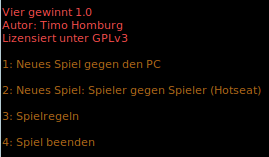
\includegraphics[width=0.9\linewidth]{img/menu.png}
		\caption{Spielmenü}
		\label{fig:sub1}
	\end{subfigure}%
	\begin{subfigure}{.5\textwidth}
		\centering
		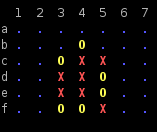
\includegraphics[width=0.9\linewidth]{img/connectfour.png}
		\caption{Spielbildschirm}
		\label{fig:sub2}
	\end{subfigure}
	\label{fig:test}
\end{figure}
\begin{figure}
	\centering
	\begin{subfigure}{.5\textwidth}
		\centering
		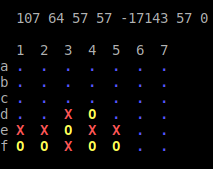
\includegraphics[width=0.9\linewidth]{img/debugmode.png}
		\caption{Debug Modus}
		\label{fig:sub3}
	\end{subfigure}%
	\begin{subfigure}{.5\textwidth}
		\centering
		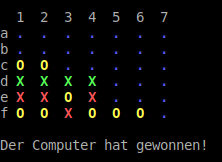
\includegraphics[width=0.9\linewidth]{img/computerwon.png}
		\caption{Der Computer hat gewonnen}
		\label{fig:sub4}
	\end{subfigure}
	\label{fig:test}
\end{figure}
\end{document}
